\begin{figure*}[h]
  \centering
  % 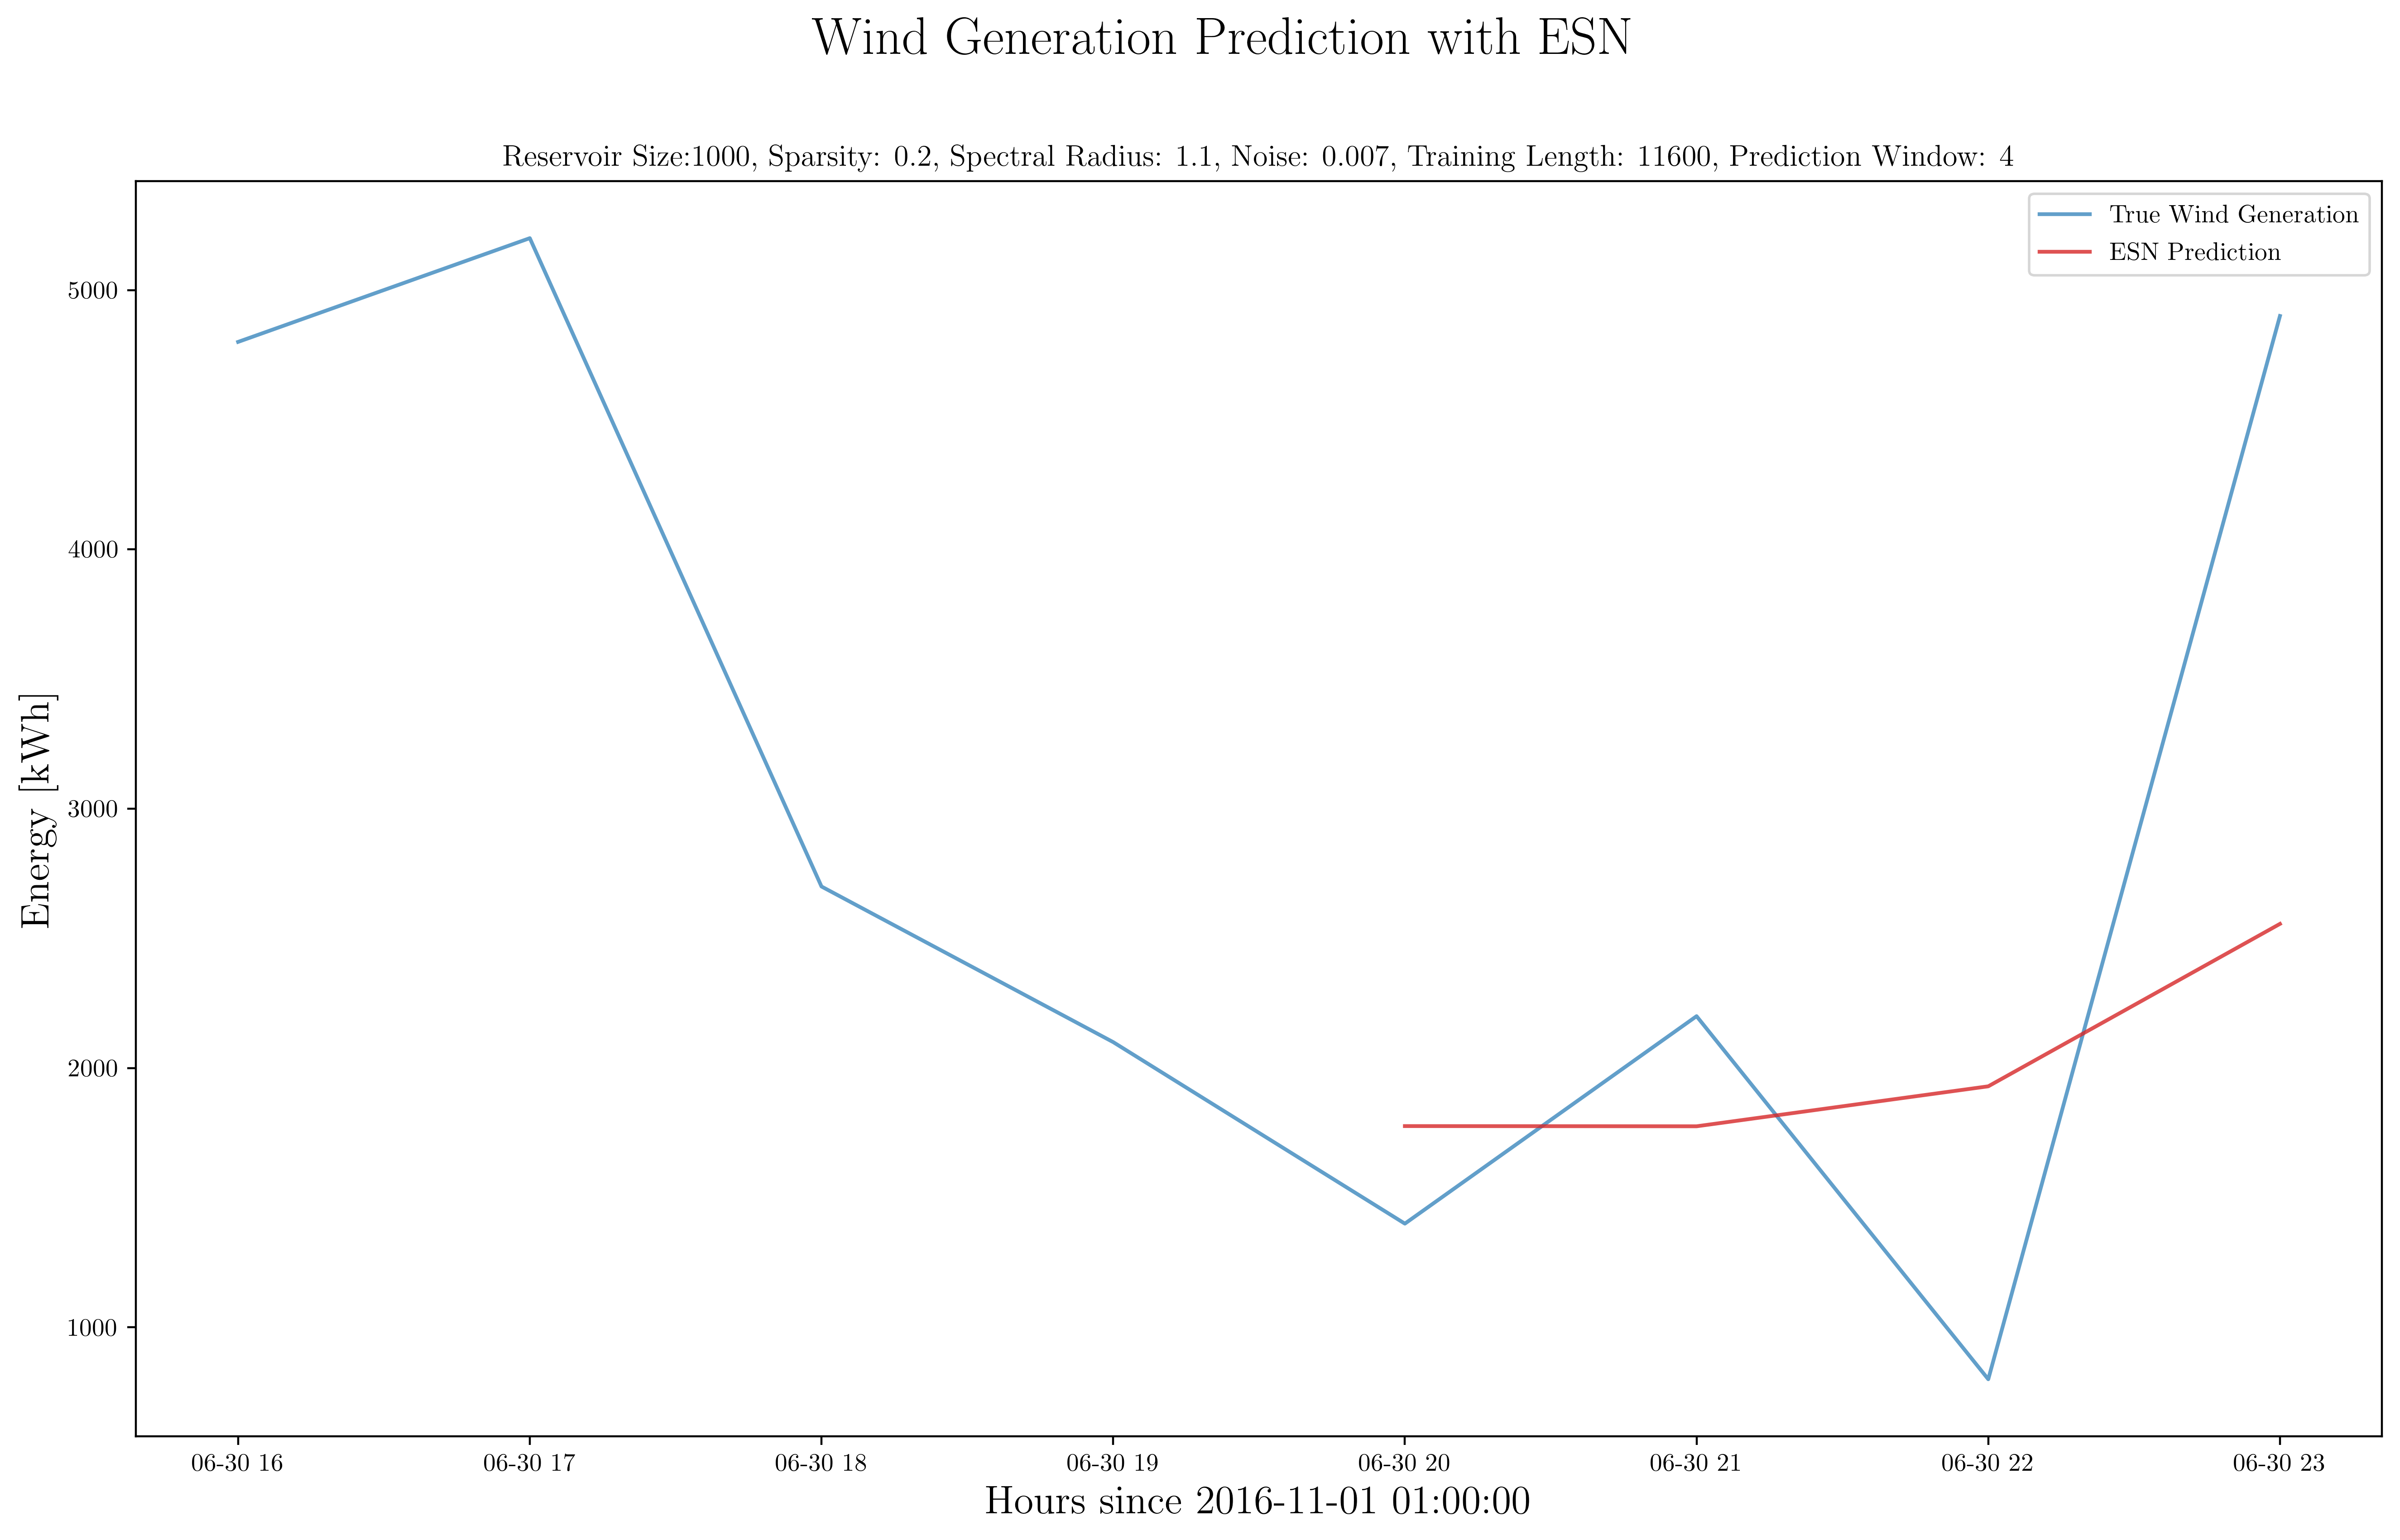
\includegraphics[width=0.8\textwidth]{04_wind_wettemp_prediction.png}
  %% Creator: Matplotlib, PGF backend
%%
%% To include the figure in your LaTeX document, write
%%   \input{<filename>.pgf}
%%
%% Make sure the required packages are loaded in your preamble
%%   \usepackage{pgf}
%%
%% Figures using additional raster images can only be included by \input if
%% they are in the same directory as the main LaTeX file. For loading figures
%% from other directories you can use the `import` package
%%   \usepackage{import}
%% and then include the figures with
%%   \import{<path to file>}{<filename>.pgf}
%%
%% Matplotlib used the following preamble
%%
\begingroup%
\makeatletter%
\begin{pgfpicture}%
\pgfpathrectangle{\pgfpointorigin}{\pgfqpoint{5.531696in}{3.164528in}}%
\pgfusepath{use as bounding box, clip}%
\begin{pgfscope}%
\pgfsetbuttcap%
\pgfsetmiterjoin%
\definecolor{currentfill}{rgb}{1.000000,1.000000,1.000000}%
\pgfsetfillcolor{currentfill}%
\pgfsetlinewidth{0.000000pt}%
\definecolor{currentstroke}{rgb}{1.000000,1.000000,1.000000}%
\pgfsetstrokecolor{currentstroke}%
\pgfsetdash{}{0pt}%
\pgfpathmoveto{\pgfqpoint{0.000000in}{0.000000in}}%
\pgfpathlineto{\pgfqpoint{5.531696in}{0.000000in}}%
\pgfpathlineto{\pgfqpoint{5.531696in}{3.164528in}}%
\pgfpathlineto{\pgfqpoint{0.000000in}{3.164528in}}%
\pgfpathclose%
\pgfusepath{fill}%
\end{pgfscope}%
\begin{pgfscope}%
\pgfsetbuttcap%
\pgfsetmiterjoin%
\definecolor{currentfill}{rgb}{1.000000,1.000000,1.000000}%
\pgfsetfillcolor{currentfill}%
\pgfsetlinewidth{0.000000pt}%
\definecolor{currentstroke}{rgb}{0.000000,0.000000,0.000000}%
\pgfsetstrokecolor{currentstroke}%
\pgfsetstrokeopacity{0.000000}%
\pgfsetdash{}{0pt}%
\pgfpathmoveto{\pgfqpoint{0.669445in}{0.499691in}}%
\pgfpathlineto{\pgfqpoint{5.431696in}{0.499691in}}%
\pgfpathlineto{\pgfqpoint{5.431696in}{2.865455in}}%
\pgfpathlineto{\pgfqpoint{0.669445in}{2.865455in}}%
\pgfpathclose%
\pgfusepath{fill}%
\end{pgfscope}%
\begin{pgfscope}%
\pgfpathrectangle{\pgfqpoint{0.669445in}{0.499691in}}{\pgfqpoint{4.762251in}{2.365763in}}%
\pgfusepath{clip}%
\pgfsetbuttcap%
\pgfsetroundjoin%
\definecolor{currentfill}{rgb}{0.501961,0.501961,0.501961}%
\pgfsetfillcolor{currentfill}%
\pgfsetfillopacity{0.600000}%
\pgfsetlinewidth{1.003750pt}%
\definecolor{currentstroke}{rgb}{0.501961,0.501961,0.501961}%
\pgfsetstrokecolor{currentstroke}%
\pgfsetstrokeopacity{0.600000}%
\pgfsetdash{}{0pt}%
\pgfpathmoveto{\pgfqpoint{3.711362in}{0.628500in}}%
\pgfpathlineto{\pgfqpoint{3.711362in}{0.664695in}}%
\pgfpathlineto{\pgfqpoint{3.756933in}{0.664695in}}%
\pgfpathlineto{\pgfqpoint{3.756933in}{0.607226in}}%
\pgfpathlineto{\pgfqpoint{3.756933in}{0.607226in}}%
\pgfpathlineto{\pgfqpoint{3.711362in}{0.628500in}}%
\pgfpathclose%
\pgfusepath{stroke,fill}%
\end{pgfscope}%
\begin{pgfscope}%
\pgfsetbuttcap%
\pgfsetroundjoin%
\definecolor{currentfill}{rgb}{0.000000,0.000000,0.000000}%
\pgfsetfillcolor{currentfill}%
\pgfsetlinewidth{0.803000pt}%
\definecolor{currentstroke}{rgb}{0.000000,0.000000,0.000000}%
\pgfsetstrokecolor{currentstroke}%
\pgfsetdash{}{0pt}%
\pgfsys@defobject{currentmarker}{\pgfqpoint{0.000000in}{-0.048611in}}{\pgfqpoint{0.000000in}{0.000000in}}{%
\pgfpathmoveto{\pgfqpoint{0.000000in}{0.000000in}}%
\pgfpathlineto{\pgfqpoint{0.000000in}{-0.048611in}}%
\pgfusepath{stroke,fill}%
}%
\begin{pgfscope}%
\pgfsys@transformshift{1.250485in}{0.499691in}%
\pgfsys@useobject{currentmarker}{}%
\end{pgfscope}%
\end{pgfscope}%
\begin{pgfscope}%
\definecolor{textcolor}{rgb}{0.000000,0.000000,0.000000}%
\pgfsetstrokecolor{textcolor}%
\pgfsetfillcolor{textcolor}%
\pgftext[x=1.250485in,y=0.402469in,,top]{\color{textcolor}\rmfamily\fontsize{10.000000}{12.000000}\selectfont \(\displaystyle 23240\)}%
\end{pgfscope}%
\begin{pgfscope}%
\pgfsetbuttcap%
\pgfsetroundjoin%
\definecolor{currentfill}{rgb}{0.000000,0.000000,0.000000}%
\pgfsetfillcolor{currentfill}%
\pgfsetlinewidth{0.803000pt}%
\definecolor{currentstroke}{rgb}{0.000000,0.000000,0.000000}%
\pgfsetstrokecolor{currentstroke}%
\pgfsetdash{}{0pt}%
\pgfsys@defobject{currentmarker}{\pgfqpoint{0.000000in}{-0.048611in}}{\pgfqpoint{0.000000in}{0.000000in}}{%
\pgfpathmoveto{\pgfqpoint{0.000000in}{0.000000in}}%
\pgfpathlineto{\pgfqpoint{0.000000in}{-0.048611in}}%
\pgfusepath{stroke,fill}%
}%
\begin{pgfscope}%
\pgfsys@transformshift{2.161921in}{0.499691in}%
\pgfsys@useobject{currentmarker}{}%
\end{pgfscope}%
\end{pgfscope}%
\begin{pgfscope}%
\definecolor{textcolor}{rgb}{0.000000,0.000000,0.000000}%
\pgfsetstrokecolor{textcolor}%
\pgfsetfillcolor{textcolor}%
\pgftext[x=2.161921in,y=0.402469in,,top]{\color{textcolor}\rmfamily\fontsize{10.000000}{12.000000}\selectfont \(\displaystyle 23260\)}%
\end{pgfscope}%
\begin{pgfscope}%
\pgfsetbuttcap%
\pgfsetroundjoin%
\definecolor{currentfill}{rgb}{0.000000,0.000000,0.000000}%
\pgfsetfillcolor{currentfill}%
\pgfsetlinewidth{0.803000pt}%
\definecolor{currentstroke}{rgb}{0.000000,0.000000,0.000000}%
\pgfsetstrokecolor{currentstroke}%
\pgfsetdash{}{0pt}%
\pgfsys@defobject{currentmarker}{\pgfqpoint{0.000000in}{-0.048611in}}{\pgfqpoint{0.000000in}{0.000000in}}{%
\pgfpathmoveto{\pgfqpoint{0.000000in}{0.000000in}}%
\pgfpathlineto{\pgfqpoint{0.000000in}{-0.048611in}}%
\pgfusepath{stroke,fill}%
}%
\begin{pgfscope}%
\pgfsys@transformshift{3.073357in}{0.499691in}%
\pgfsys@useobject{currentmarker}{}%
\end{pgfscope}%
\end{pgfscope}%
\begin{pgfscope}%
\definecolor{textcolor}{rgb}{0.000000,0.000000,0.000000}%
\pgfsetstrokecolor{textcolor}%
\pgfsetfillcolor{textcolor}%
\pgftext[x=3.073357in,y=0.402469in,,top]{\color{textcolor}\rmfamily\fontsize{10.000000}{12.000000}\selectfont \(\displaystyle 23280\)}%
\end{pgfscope}%
\begin{pgfscope}%
\pgfsetbuttcap%
\pgfsetroundjoin%
\definecolor{currentfill}{rgb}{0.000000,0.000000,0.000000}%
\pgfsetfillcolor{currentfill}%
\pgfsetlinewidth{0.803000pt}%
\definecolor{currentstroke}{rgb}{0.000000,0.000000,0.000000}%
\pgfsetstrokecolor{currentstroke}%
\pgfsetdash{}{0pt}%
\pgfsys@defobject{currentmarker}{\pgfqpoint{0.000000in}{-0.048611in}}{\pgfqpoint{0.000000in}{0.000000in}}{%
\pgfpathmoveto{\pgfqpoint{0.000000in}{0.000000in}}%
\pgfpathlineto{\pgfqpoint{0.000000in}{-0.048611in}}%
\pgfusepath{stroke,fill}%
}%
\begin{pgfscope}%
\pgfsys@transformshift{3.984792in}{0.499691in}%
\pgfsys@useobject{currentmarker}{}%
\end{pgfscope}%
\end{pgfscope}%
\begin{pgfscope}%
\definecolor{textcolor}{rgb}{0.000000,0.000000,0.000000}%
\pgfsetstrokecolor{textcolor}%
\pgfsetfillcolor{textcolor}%
\pgftext[x=3.984792in,y=0.402469in,,top]{\color{textcolor}\rmfamily\fontsize{10.000000}{12.000000}\selectfont \(\displaystyle 23300\)}%
\end{pgfscope}%
\begin{pgfscope}%
\pgfsetbuttcap%
\pgfsetroundjoin%
\definecolor{currentfill}{rgb}{0.000000,0.000000,0.000000}%
\pgfsetfillcolor{currentfill}%
\pgfsetlinewidth{0.803000pt}%
\definecolor{currentstroke}{rgb}{0.000000,0.000000,0.000000}%
\pgfsetstrokecolor{currentstroke}%
\pgfsetdash{}{0pt}%
\pgfsys@defobject{currentmarker}{\pgfqpoint{0.000000in}{-0.048611in}}{\pgfqpoint{0.000000in}{0.000000in}}{%
\pgfpathmoveto{\pgfqpoint{0.000000in}{0.000000in}}%
\pgfpathlineto{\pgfqpoint{0.000000in}{-0.048611in}}%
\pgfusepath{stroke,fill}%
}%
\begin{pgfscope}%
\pgfsys@transformshift{4.896228in}{0.499691in}%
\pgfsys@useobject{currentmarker}{}%
\end{pgfscope}%
\end{pgfscope}%
\begin{pgfscope}%
\definecolor{textcolor}{rgb}{0.000000,0.000000,0.000000}%
\pgfsetstrokecolor{textcolor}%
\pgfsetfillcolor{textcolor}%
\pgftext[x=4.896228in,y=0.402469in,,top]{\color{textcolor}\rmfamily\fontsize{10.000000}{12.000000}\selectfont \(\displaystyle 23320\)}%
\end{pgfscope}%
\begin{pgfscope}%
\definecolor{textcolor}{rgb}{0.000000,0.000000,0.000000}%
\pgfsetstrokecolor{textcolor}%
\pgfsetfillcolor{textcolor}%
\pgftext[x=3.050571in,y=0.223457in,,top]{\color{textcolor}\rmfamily\fontsize{10.000000}{12.000000}\selectfont Hours since 2016-11-01 01:00:00}%
\end{pgfscope}%
\begin{pgfscope}%
\pgfsetbuttcap%
\pgfsetroundjoin%
\definecolor{currentfill}{rgb}{0.000000,0.000000,0.000000}%
\pgfsetfillcolor{currentfill}%
\pgfsetlinewidth{0.803000pt}%
\definecolor{currentstroke}{rgb}{0.000000,0.000000,0.000000}%
\pgfsetstrokecolor{currentstroke}%
\pgfsetdash{}{0pt}%
\pgfsys@defobject{currentmarker}{\pgfqpoint{-0.048611in}{0.000000in}}{\pgfqpoint{0.000000in}{0.000000in}}{%
\pgfpathmoveto{\pgfqpoint{0.000000in}{0.000000in}}%
\pgfpathlineto{\pgfqpoint{-0.048611in}{0.000000in}}%
\pgfusepath{stroke,fill}%
}%
\begin{pgfscope}%
\pgfsys@transformshift{0.669445in}{0.664695in}%
\pgfsys@useobject{currentmarker}{}%
\end{pgfscope}%
\end{pgfscope}%
\begin{pgfscope}%
\definecolor{textcolor}{rgb}{0.000000,0.000000,0.000000}%
\pgfsetstrokecolor{textcolor}%
\pgfsetfillcolor{textcolor}%
\pgftext[x=0.502778in,y=0.616470in,left,base]{\color{textcolor}\rmfamily\fontsize{10.000000}{12.000000}\selectfont \(\displaystyle 0\)}%
\end{pgfscope}%
\begin{pgfscope}%
\pgfsetbuttcap%
\pgfsetroundjoin%
\definecolor{currentfill}{rgb}{0.000000,0.000000,0.000000}%
\pgfsetfillcolor{currentfill}%
\pgfsetlinewidth{0.803000pt}%
\definecolor{currentstroke}{rgb}{0.000000,0.000000,0.000000}%
\pgfsetstrokecolor{currentstroke}%
\pgfsetdash{}{0pt}%
\pgfsys@defobject{currentmarker}{\pgfqpoint{-0.048611in}{0.000000in}}{\pgfqpoint{0.000000in}{0.000000in}}{%
\pgfpathmoveto{\pgfqpoint{0.000000in}{0.000000in}}%
\pgfpathlineto{\pgfqpoint{-0.048611in}{0.000000in}}%
\pgfusepath{stroke,fill}%
}%
\begin{pgfscope}%
\pgfsys@transformshift{0.669445in}{1.031927in}%
\pgfsys@useobject{currentmarker}{}%
\end{pgfscope}%
\end{pgfscope}%
\begin{pgfscope}%
\definecolor{textcolor}{rgb}{0.000000,0.000000,0.000000}%
\pgfsetstrokecolor{textcolor}%
\pgfsetfillcolor{textcolor}%
\pgftext[x=0.294444in,y=0.983702in,left,base]{\color{textcolor}\rmfamily\fontsize{10.000000}{12.000000}\selectfont \(\displaystyle 1000\)}%
\end{pgfscope}%
\begin{pgfscope}%
\pgfsetbuttcap%
\pgfsetroundjoin%
\definecolor{currentfill}{rgb}{0.000000,0.000000,0.000000}%
\pgfsetfillcolor{currentfill}%
\pgfsetlinewidth{0.803000pt}%
\definecolor{currentstroke}{rgb}{0.000000,0.000000,0.000000}%
\pgfsetstrokecolor{currentstroke}%
\pgfsetdash{}{0pt}%
\pgfsys@defobject{currentmarker}{\pgfqpoint{-0.048611in}{0.000000in}}{\pgfqpoint{0.000000in}{0.000000in}}{%
\pgfpathmoveto{\pgfqpoint{0.000000in}{0.000000in}}%
\pgfpathlineto{\pgfqpoint{-0.048611in}{0.000000in}}%
\pgfusepath{stroke,fill}%
}%
\begin{pgfscope}%
\pgfsys@transformshift{0.669445in}{1.399160in}%
\pgfsys@useobject{currentmarker}{}%
\end{pgfscope}%
\end{pgfscope}%
\begin{pgfscope}%
\definecolor{textcolor}{rgb}{0.000000,0.000000,0.000000}%
\pgfsetstrokecolor{textcolor}%
\pgfsetfillcolor{textcolor}%
\pgftext[x=0.294444in,y=1.350935in,left,base]{\color{textcolor}\rmfamily\fontsize{10.000000}{12.000000}\selectfont \(\displaystyle 2000\)}%
\end{pgfscope}%
\begin{pgfscope}%
\pgfsetbuttcap%
\pgfsetroundjoin%
\definecolor{currentfill}{rgb}{0.000000,0.000000,0.000000}%
\pgfsetfillcolor{currentfill}%
\pgfsetlinewidth{0.803000pt}%
\definecolor{currentstroke}{rgb}{0.000000,0.000000,0.000000}%
\pgfsetstrokecolor{currentstroke}%
\pgfsetdash{}{0pt}%
\pgfsys@defobject{currentmarker}{\pgfqpoint{-0.048611in}{0.000000in}}{\pgfqpoint{0.000000in}{0.000000in}}{%
\pgfpathmoveto{\pgfqpoint{0.000000in}{0.000000in}}%
\pgfpathlineto{\pgfqpoint{-0.048611in}{0.000000in}}%
\pgfusepath{stroke,fill}%
}%
\begin{pgfscope}%
\pgfsys@transformshift{0.669445in}{1.766392in}%
\pgfsys@useobject{currentmarker}{}%
\end{pgfscope}%
\end{pgfscope}%
\begin{pgfscope}%
\definecolor{textcolor}{rgb}{0.000000,0.000000,0.000000}%
\pgfsetstrokecolor{textcolor}%
\pgfsetfillcolor{textcolor}%
\pgftext[x=0.294444in,y=1.718167in,left,base]{\color{textcolor}\rmfamily\fontsize{10.000000}{12.000000}\selectfont \(\displaystyle 3000\)}%
\end{pgfscope}%
\begin{pgfscope}%
\pgfsetbuttcap%
\pgfsetroundjoin%
\definecolor{currentfill}{rgb}{0.000000,0.000000,0.000000}%
\pgfsetfillcolor{currentfill}%
\pgfsetlinewidth{0.803000pt}%
\definecolor{currentstroke}{rgb}{0.000000,0.000000,0.000000}%
\pgfsetstrokecolor{currentstroke}%
\pgfsetdash{}{0pt}%
\pgfsys@defobject{currentmarker}{\pgfqpoint{-0.048611in}{0.000000in}}{\pgfqpoint{0.000000in}{0.000000in}}{%
\pgfpathmoveto{\pgfqpoint{0.000000in}{0.000000in}}%
\pgfpathlineto{\pgfqpoint{-0.048611in}{0.000000in}}%
\pgfusepath{stroke,fill}%
}%
\begin{pgfscope}%
\pgfsys@transformshift{0.669445in}{2.133625in}%
\pgfsys@useobject{currentmarker}{}%
\end{pgfscope}%
\end{pgfscope}%
\begin{pgfscope}%
\definecolor{textcolor}{rgb}{0.000000,0.000000,0.000000}%
\pgfsetstrokecolor{textcolor}%
\pgfsetfillcolor{textcolor}%
\pgftext[x=0.294444in,y=2.085399in,left,base]{\color{textcolor}\rmfamily\fontsize{10.000000}{12.000000}\selectfont \(\displaystyle 4000\)}%
\end{pgfscope}%
\begin{pgfscope}%
\pgfsetbuttcap%
\pgfsetroundjoin%
\definecolor{currentfill}{rgb}{0.000000,0.000000,0.000000}%
\pgfsetfillcolor{currentfill}%
\pgfsetlinewidth{0.803000pt}%
\definecolor{currentstroke}{rgb}{0.000000,0.000000,0.000000}%
\pgfsetstrokecolor{currentstroke}%
\pgfsetdash{}{0pt}%
\pgfsys@defobject{currentmarker}{\pgfqpoint{-0.048611in}{0.000000in}}{\pgfqpoint{0.000000in}{0.000000in}}{%
\pgfpathmoveto{\pgfqpoint{0.000000in}{0.000000in}}%
\pgfpathlineto{\pgfqpoint{-0.048611in}{0.000000in}}%
\pgfusepath{stroke,fill}%
}%
\begin{pgfscope}%
\pgfsys@transformshift{0.669445in}{2.500857in}%
\pgfsys@useobject{currentmarker}{}%
\end{pgfscope}%
\end{pgfscope}%
\begin{pgfscope}%
\definecolor{textcolor}{rgb}{0.000000,0.000000,0.000000}%
\pgfsetstrokecolor{textcolor}%
\pgfsetfillcolor{textcolor}%
\pgftext[x=0.294444in,y=2.452632in,left,base]{\color{textcolor}\rmfamily\fontsize{10.000000}{12.000000}\selectfont \(\displaystyle 5000\)}%
\end{pgfscope}%
\begin{pgfscope}%
\definecolor{textcolor}{rgb}{0.000000,0.000000,0.000000}%
\pgfsetstrokecolor{textcolor}%
\pgfsetfillcolor{textcolor}%
\pgftext[x=0.238889in,y=1.682573in,,bottom,rotate=90.000000]{\color{textcolor}\rmfamily\fontsize{10.000000}{12.000000}\selectfont Energy [kWh]}%
\end{pgfscope}%
\begin{pgfscope}%
\pgfpathrectangle{\pgfqpoint{0.669445in}{0.499691in}}{\pgfqpoint{4.762251in}{2.365763in}}%
\pgfusepath{clip}%
\pgfsetrectcap%
\pgfsetroundjoin%
\pgfsetlinewidth{1.505625pt}%
\definecolor{currentstroke}{rgb}{0.121569,0.466667,0.705882}%
\pgfsetstrokecolor{currentstroke}%
\pgfsetstrokeopacity{0.700000}%
\pgfsetdash{}{0pt}%
\pgfpathmoveto{\pgfqpoint{0.885911in}{1.215544in}}%
\pgfpathlineto{\pgfqpoint{0.931483in}{1.288990in}}%
\pgfpathlineto{\pgfqpoint{0.977055in}{1.105374in}}%
\pgfpathlineto{\pgfqpoint{1.022627in}{0.848311in}}%
\pgfpathlineto{\pgfqpoint{1.068198in}{0.885034in}}%
\pgfpathlineto{\pgfqpoint{1.113770in}{1.105374in}}%
\pgfpathlineto{\pgfqpoint{1.159342in}{0.995204in}}%
\pgfpathlineto{\pgfqpoint{1.204914in}{0.995204in}}%
\pgfpathlineto{\pgfqpoint{1.250485in}{0.738141in}}%
\pgfpathlineto{\pgfqpoint{1.296057in}{0.701418in}}%
\pgfpathlineto{\pgfqpoint{1.341629in}{0.701418in}}%
\pgfpathlineto{\pgfqpoint{1.387201in}{0.774865in}}%
\pgfpathlineto{\pgfqpoint{1.432773in}{0.701418in}}%
\pgfpathlineto{\pgfqpoint{1.478344in}{0.811588in}}%
\pgfpathlineto{\pgfqpoint{1.523916in}{0.848311in}}%
\pgfpathlineto{\pgfqpoint{1.569488in}{0.995204in}}%
\pgfpathlineto{\pgfqpoint{1.615060in}{0.885034in}}%
\pgfpathlineto{\pgfqpoint{1.660631in}{1.031927in}}%
\pgfpathlineto{\pgfqpoint{1.706203in}{0.921758in}}%
\pgfpathlineto{\pgfqpoint{1.751775in}{0.774865in}}%
\pgfpathlineto{\pgfqpoint{1.797347in}{0.738141in}}%
\pgfpathlineto{\pgfqpoint{1.842919in}{1.215544in}}%
\pgfpathlineto{\pgfqpoint{1.888490in}{1.546053in}}%
\pgfpathlineto{\pgfqpoint{1.934062in}{1.435883in}}%
\pgfpathlineto{\pgfqpoint{1.979634in}{1.950008in}}%
\pgfpathlineto{\pgfqpoint{2.025206in}{2.757920in}}%
\pgfpathlineto{\pgfqpoint{2.070778in}{2.684473in}}%
\pgfpathlineto{\pgfqpoint{2.116349in}{2.060178in}}%
\pgfpathlineto{\pgfqpoint{2.161921in}{1.288990in}}%
\pgfpathlineto{\pgfqpoint{2.207493in}{1.288990in}}%
\pgfpathlineto{\pgfqpoint{2.253065in}{1.729669in}}%
\pgfpathlineto{\pgfqpoint{2.298636in}{1.546053in}}%
\pgfpathlineto{\pgfqpoint{2.344208in}{1.215544in}}%
\pgfpathlineto{\pgfqpoint{2.389780in}{1.325713in}}%
\pgfpathlineto{\pgfqpoint{2.435352in}{0.848311in}}%
\pgfpathlineto{\pgfqpoint{2.480924in}{0.664695in}}%
\pgfpathlineto{\pgfqpoint{2.526495in}{0.701418in}}%
\pgfpathlineto{\pgfqpoint{2.572067in}{0.995204in}}%
\pgfpathlineto{\pgfqpoint{2.617639in}{1.582776in}}%
\pgfpathlineto{\pgfqpoint{2.663211in}{1.546053in}}%
\pgfpathlineto{\pgfqpoint{2.708782in}{1.399160in}}%
\pgfpathlineto{\pgfqpoint{2.754354in}{1.472606in}}%
\pgfpathlineto{\pgfqpoint{2.799926in}{1.105374in}}%
\pgfpathlineto{\pgfqpoint{2.845498in}{1.105374in}}%
\pgfpathlineto{\pgfqpoint{2.891070in}{0.885034in}}%
\pgfpathlineto{\pgfqpoint{2.936641in}{0.664695in}}%
\pgfpathlineto{\pgfqpoint{2.982213in}{0.664695in}}%
\pgfpathlineto{\pgfqpoint{3.027785in}{0.664695in}}%
\pgfpathlineto{\pgfqpoint{3.073357in}{0.664695in}}%
\pgfpathlineto{\pgfqpoint{3.118928in}{0.664695in}}%
\pgfpathlineto{\pgfqpoint{3.164500in}{1.142097in}}%
\pgfpathlineto{\pgfqpoint{3.210072in}{1.435883in}}%
\pgfpathlineto{\pgfqpoint{3.255644in}{1.435883in}}%
\pgfpathlineto{\pgfqpoint{3.301216in}{1.399160in}}%
\pgfpathlineto{\pgfqpoint{3.346787in}{1.362437in}}%
\pgfpathlineto{\pgfqpoint{3.392359in}{1.215544in}}%
\pgfpathlineto{\pgfqpoint{3.437931in}{0.995204in}}%
\pgfpathlineto{\pgfqpoint{3.483503in}{0.921758in}}%
\pgfpathlineto{\pgfqpoint{3.529074in}{0.921758in}}%
\pgfpathlineto{\pgfqpoint{3.574646in}{0.921758in}}%
\pgfpathlineto{\pgfqpoint{3.620218in}{0.848311in}}%
\pgfpathlineto{\pgfqpoint{3.665790in}{0.811588in}}%
\pgfpathlineto{\pgfqpoint{3.711362in}{0.774865in}}%
\pgfpathlineto{\pgfqpoint{3.756933in}{0.811588in}}%
\pgfpathlineto{\pgfqpoint{3.802505in}{0.995204in}}%
\pgfpathlineto{\pgfqpoint{3.848077in}{1.031927in}}%
\pgfpathlineto{\pgfqpoint{3.893649in}{1.031927in}}%
\pgfpathlineto{\pgfqpoint{3.939220in}{1.068651in}}%
\pgfpathlineto{\pgfqpoint{3.984792in}{1.142097in}}%
\pgfpathlineto{\pgfqpoint{4.030364in}{1.325713in}}%
\pgfpathlineto{\pgfqpoint{4.075936in}{1.362437in}}%
\pgfpathlineto{\pgfqpoint{4.121508in}{1.876562in}}%
\pgfpathlineto{\pgfqpoint{4.167079in}{2.060178in}}%
\pgfpathlineto{\pgfqpoint{4.212651in}{1.546053in}}%
\pgfpathlineto{\pgfqpoint{4.258223in}{1.435883in}}%
\pgfpathlineto{\pgfqpoint{4.303795in}{1.435883in}}%
\pgfpathlineto{\pgfqpoint{4.349367in}{1.362437in}}%
\pgfpathlineto{\pgfqpoint{4.394938in}{1.288990in}}%
\pgfpathlineto{\pgfqpoint{4.440510in}{1.509330in}}%
\pgfpathlineto{\pgfqpoint{4.486082in}{1.288990in}}%
\pgfpathlineto{\pgfqpoint{4.531654in}{0.921758in}}%
\pgfpathlineto{\pgfqpoint{4.577225in}{0.885034in}}%
\pgfpathlineto{\pgfqpoint{4.622797in}{0.848311in}}%
\pgfpathlineto{\pgfqpoint{4.668369in}{0.811588in}}%
\pgfpathlineto{\pgfqpoint{4.713941in}{0.738141in}}%
\pgfpathlineto{\pgfqpoint{4.759513in}{0.738141in}}%
\pgfpathlineto{\pgfqpoint{4.805084in}{0.738141in}}%
\pgfpathlineto{\pgfqpoint{4.850656in}{0.921758in}}%
\pgfpathlineto{\pgfqpoint{4.896228in}{2.427411in}}%
\pgfpathlineto{\pgfqpoint{4.941800in}{2.574304in}}%
\pgfpathlineto{\pgfqpoint{4.987371in}{1.656223in}}%
\pgfpathlineto{\pgfqpoint{5.032943in}{1.435883in}}%
\pgfpathlineto{\pgfqpoint{5.078515in}{1.178820in}}%
\pgfpathlineto{\pgfqpoint{5.124087in}{1.472606in}}%
\pgfpathlineto{\pgfqpoint{5.169659in}{0.958481in}}%
\pgfpathlineto{\pgfqpoint{5.215230in}{2.464134in}}%
\pgfusepath{stroke}%
\end{pgfscope}%
\begin{pgfscope}%
\pgfpathrectangle{\pgfqpoint{0.669445in}{0.499691in}}{\pgfqpoint{4.762251in}{2.365763in}}%
\pgfusepath{clip}%
\pgfsetrectcap%
\pgfsetroundjoin%
\pgfsetlinewidth{1.505625pt}%
\definecolor{currentstroke}{rgb}{0.839216,0.152941,0.156863}%
\pgfsetstrokecolor{currentstroke}%
\pgfsetstrokeopacity{0.800000}%
\pgfsetdash{}{0pt}%
\pgfpathmoveto{\pgfqpoint{3.073357in}{0.753795in}}%
\pgfpathlineto{\pgfqpoint{3.118928in}{0.948254in}}%
\pgfpathlineto{\pgfqpoint{3.164500in}{1.157699in}}%
\pgfpathlineto{\pgfqpoint{3.210072in}{1.283027in}}%
\pgfpathlineto{\pgfqpoint{3.255644in}{1.438228in}}%
\pgfpathlineto{\pgfqpoint{3.301216in}{1.453076in}}%
\pgfpathlineto{\pgfqpoint{3.346787in}{1.405019in}}%
\pgfpathlineto{\pgfqpoint{3.392359in}{1.351413in}}%
\pgfpathlineto{\pgfqpoint{3.437931in}{1.147807in}}%
\pgfpathlineto{\pgfqpoint{3.483503in}{1.218688in}}%
\pgfpathlineto{\pgfqpoint{3.529074in}{1.181614in}}%
\pgfpathlineto{\pgfqpoint{3.574646in}{0.989220in}}%
\pgfpathlineto{\pgfqpoint{3.620218in}{0.772071in}}%
\pgfpathlineto{\pgfqpoint{3.665790in}{0.678363in}}%
\pgfpathlineto{\pgfqpoint{3.711362in}{0.628500in}}%
\pgfpathlineto{\pgfqpoint{3.756933in}{0.607226in}}%
\pgfpathlineto{\pgfqpoint{3.802505in}{0.804786in}}%
\pgfpathlineto{\pgfqpoint{3.848077in}{0.832314in}}%
\pgfpathlineto{\pgfqpoint{3.893649in}{0.956738in}}%
\pgfpathlineto{\pgfqpoint{3.939220in}{1.149635in}}%
\pgfpathlineto{\pgfqpoint{3.984792in}{1.162268in}}%
\pgfpathlineto{\pgfqpoint{4.030364in}{1.119773in}}%
\pgfpathlineto{\pgfqpoint{4.075936in}{1.163592in}}%
\pgfpathlineto{\pgfqpoint{4.121508in}{1.157439in}}%
\pgfpathlineto{\pgfqpoint{4.167079in}{2.103300in}}%
\pgfpathlineto{\pgfqpoint{4.212651in}{2.048643in}}%
\pgfpathlineto{\pgfqpoint{4.258223in}{2.047799in}}%
\pgfpathlineto{\pgfqpoint{4.303795in}{1.955583in}}%
\pgfpathlineto{\pgfqpoint{4.349367in}{1.362093in}}%
\pgfpathlineto{\pgfqpoint{4.394938in}{1.243529in}}%
\pgfpathlineto{\pgfqpoint{4.440510in}{1.077970in}}%
\pgfpathlineto{\pgfqpoint{4.486082in}{1.001823in}}%
\pgfpathlineto{\pgfqpoint{4.531654in}{1.041847in}}%
\pgfpathlineto{\pgfqpoint{4.577225in}{0.951794in}}%
\pgfpathlineto{\pgfqpoint{4.622797in}{0.892875in}}%
\pgfpathlineto{\pgfqpoint{4.668369in}{0.767402in}}%
\pgfpathlineto{\pgfqpoint{4.713941in}{0.774508in}}%
\pgfpathlineto{\pgfqpoint{4.759513in}{0.818697in}}%
\pgfpathlineto{\pgfqpoint{4.805084in}{0.757482in}}%
\pgfpathlineto{\pgfqpoint{4.850656in}{0.801801in}}%
\pgfpathlineto{\pgfqpoint{4.896228in}{2.357373in}}%
\pgfpathlineto{\pgfqpoint{4.941800in}{2.663398in}}%
\pgfpathlineto{\pgfqpoint{4.987371in}{1.893177in}}%
\pgfpathlineto{\pgfqpoint{5.032943in}{1.314311in}}%
\pgfpathlineto{\pgfqpoint{5.078515in}{1.189779in}}%
\pgfpathlineto{\pgfqpoint{5.124087in}{1.418964in}}%
\pgfpathlineto{\pgfqpoint{5.169659in}{1.717752in}}%
\pgfpathlineto{\pgfqpoint{5.215230in}{1.729050in}}%
\pgfusepath{stroke}%
\end{pgfscope}%
\begin{pgfscope}%
\pgfpathrectangle{\pgfqpoint{0.669445in}{0.499691in}}{\pgfqpoint{4.762251in}{2.365763in}}%
\pgfusepath{clip}%
\pgfsetrectcap%
\pgfsetroundjoin%
\pgfsetlinewidth{1.505625pt}%
\definecolor{currentstroke}{rgb}{0.121569,0.466667,0.705882}%
\pgfsetstrokecolor{currentstroke}%
\pgfsetstrokeopacity{0.000000}%
\pgfsetdash{}{0pt}%
\pgfpathmoveto{\pgfqpoint{0.669445in}{0.664695in}}%
\pgfpathlineto{\pgfqpoint{5.431696in}{0.664695in}}%
\pgfusepath{stroke}%
\end{pgfscope}%
\begin{pgfscope}%
\pgfsetrectcap%
\pgfsetmiterjoin%
\pgfsetlinewidth{0.803000pt}%
\definecolor{currentstroke}{rgb}{0.000000,0.000000,0.000000}%
\pgfsetstrokecolor{currentstroke}%
\pgfsetdash{}{0pt}%
\pgfpathmoveto{\pgfqpoint{0.669445in}{0.499691in}}%
\pgfpathlineto{\pgfqpoint{0.669445in}{2.865455in}}%
\pgfusepath{stroke}%
\end{pgfscope}%
\begin{pgfscope}%
\pgfsetrectcap%
\pgfsetmiterjoin%
\pgfsetlinewidth{0.803000pt}%
\definecolor{currentstroke}{rgb}{0.000000,0.000000,0.000000}%
\pgfsetstrokecolor{currentstroke}%
\pgfsetdash{}{0pt}%
\pgfpathmoveto{\pgfqpoint{5.431696in}{0.499691in}}%
\pgfpathlineto{\pgfqpoint{5.431696in}{2.865455in}}%
\pgfusepath{stroke}%
\end{pgfscope}%
\begin{pgfscope}%
\pgfsetrectcap%
\pgfsetmiterjoin%
\pgfsetlinewidth{0.803000pt}%
\definecolor{currentstroke}{rgb}{0.000000,0.000000,0.000000}%
\pgfsetstrokecolor{currentstroke}%
\pgfsetdash{}{0pt}%
\pgfpathmoveto{\pgfqpoint{0.669445in}{0.499691in}}%
\pgfpathlineto{\pgfqpoint{5.431696in}{0.499691in}}%
\pgfusepath{stroke}%
\end{pgfscope}%
\begin{pgfscope}%
\pgfsetrectcap%
\pgfsetmiterjoin%
\pgfsetlinewidth{0.803000pt}%
\definecolor{currentstroke}{rgb}{0.000000,0.000000,0.000000}%
\pgfsetstrokecolor{currentstroke}%
\pgfsetdash{}{0pt}%
\pgfpathmoveto{\pgfqpoint{0.669445in}{2.865455in}}%
\pgfpathlineto{\pgfqpoint{5.431696in}{2.865455in}}%
\pgfusepath{stroke}%
\end{pgfscope}%
\begin{pgfscope}%
\definecolor{textcolor}{rgb}{0.000000,0.000000,0.000000}%
\pgfsetstrokecolor{textcolor}%
\pgfsetfillcolor{textcolor}%
\pgftext[x=3.050571in,y=2.948788in,,base]{\color{textcolor}\rmfamily\fontsize{12.000000}{14.400000}\selectfont Wind Generation Prediction with an ESN}%
\end{pgfscope}%
\begin{pgfscope}%
\pgfsetbuttcap%
\pgfsetmiterjoin%
\definecolor{currentfill}{rgb}{1.000000,1.000000,1.000000}%
\pgfsetfillcolor{currentfill}%
\pgfsetfillopacity{0.800000}%
\pgfsetlinewidth{1.003750pt}%
\definecolor{currentstroke}{rgb}{0.800000,0.800000,0.800000}%
\pgfsetstrokecolor{currentstroke}%
\pgfsetstrokeopacity{0.800000}%
\pgfsetdash{}{0pt}%
\pgfpathmoveto{\pgfqpoint{0.766667in}{2.366998in}}%
\pgfpathlineto{\pgfqpoint{2.160574in}{2.366998in}}%
\pgfpathquadraticcurveto{\pgfqpoint{2.188352in}{2.366998in}}{\pgfqpoint{2.188352in}{2.394776in}}%
\pgfpathlineto{\pgfqpoint{2.188352in}{2.768232in}}%
\pgfpathquadraticcurveto{\pgfqpoint{2.188352in}{2.796010in}}{\pgfqpoint{2.160574in}{2.796010in}}%
\pgfpathlineto{\pgfqpoint{0.766667in}{2.796010in}}%
\pgfpathquadraticcurveto{\pgfqpoint{0.738890in}{2.796010in}}{\pgfqpoint{0.738890in}{2.768232in}}%
\pgfpathlineto{\pgfqpoint{0.738890in}{2.394776in}}%
\pgfpathquadraticcurveto{\pgfqpoint{0.738890in}{2.366998in}}{\pgfqpoint{0.766667in}{2.366998in}}%
\pgfpathclose%
\pgfusepath{stroke,fill}%
\end{pgfscope}%
\begin{pgfscope}%
\pgfsetrectcap%
\pgfsetroundjoin%
\pgfsetlinewidth{1.505625pt}%
\definecolor{currentstroke}{rgb}{0.121569,0.466667,0.705882}%
\pgfsetstrokecolor{currentstroke}%
\pgfsetstrokeopacity{0.700000}%
\pgfsetdash{}{0pt}%
\pgfpathmoveto{\pgfqpoint{0.794445in}{2.691843in}}%
\pgfpathlineto{\pgfqpoint{1.072223in}{2.691843in}}%
\pgfusepath{stroke}%
\end{pgfscope}%
\begin{pgfscope}%
\definecolor{textcolor}{rgb}{0.000000,0.000000,0.000000}%
\pgfsetstrokecolor{textcolor}%
\pgfsetfillcolor{textcolor}%
\pgftext[x=1.183334in,y=2.643232in,left,base]{\color{textcolor}\rmfamily\fontsize{10.000000}{12.000000}\selectfont True Demand}%
\end{pgfscope}%
\begin{pgfscope}%
\pgfsetrectcap%
\pgfsetroundjoin%
\pgfsetlinewidth{1.505625pt}%
\definecolor{currentstroke}{rgb}{0.839216,0.152941,0.156863}%
\pgfsetstrokecolor{currentstroke}%
\pgfsetstrokeopacity{0.800000}%
\pgfsetdash{}{0pt}%
\pgfpathmoveto{\pgfqpoint{0.794445in}{2.498171in}}%
\pgfpathlineto{\pgfqpoint{1.072223in}{2.498171in}}%
\pgfusepath{stroke}%
\end{pgfscope}%
\begin{pgfscope}%
\definecolor{textcolor}{rgb}{0.000000,0.000000,0.000000}%
\pgfsetstrokecolor{textcolor}%
\pgfsetfillcolor{textcolor}%
\pgftext[x=1.183334in,y=2.449560in,left,base]{\color{textcolor}\rmfamily\fontsize{10.000000}{12.000000}\selectfont ESN Prediction}%
\end{pgfscope}%
\end{pgfpicture}%
\makeatother%
\endgroup%

  \caption{The optimized 4 hour ahead wind energy prediction. The inputs for this forecast were wind energy and hourly windspeed. \textit{Hyperparameters}: Reservoir Size:1000, Sparsity: 0.15, Spectral Radius: 0.9, Noise: 0.001, Training Length: 14300, Prediction Window: 4, Random state: 85}
  \label{fig:wind04}
\end{figure*}
% \begin{center}
  \begin{table*}[h]
    \centering
    \caption{Tabulated error for 4-hour ahead wind forecasts with various coupled quantities. Improvement indicates the percentage improvement over the base case of forecasting wind energy alone.}
    \label{tab:wind04}
    \begin{tabular}{l|r|r|r|r|r}
      & & & & Improvement & Improvement \\
      Scenario &NRMSE & MAE & RMSE & MAE (\%) & RMSE (\%)\\
      \hline
      Wind Energy & 0.88507 &0.0903 & 0.1243 & [-] & [-] \\
      Wind + Sun Elevation & 0.83394 &0.0705 & 0.1171 & -21.9269 & -5.7924 \\
      Wind + Humidity & 0.85522 & 0.0813 & 0.1201 & -9.9668 & -3.3789 \\
      Wind + Pressure & 0.88587 & 0.0866 & 0.1244 & -4.0974 & +0.0804 \\
      Wind + Wet Bulb Temp. & 0.76203 & 0.0731 & 0.1070 & -19.0476 & -13.9179 \\
      Wind + Dry Bulb Temp. & 0.79939 & 0.0747 & 0.1123 & -17.2757 & -9.9654 \\
      Wind + Wind Speed & 0.59596 & 0.0571 & 0.0837 & -36.7663 & -32.6629 \\
    \end{tabular}
  \end{table*}
% \end{center}

\begin{figure}
  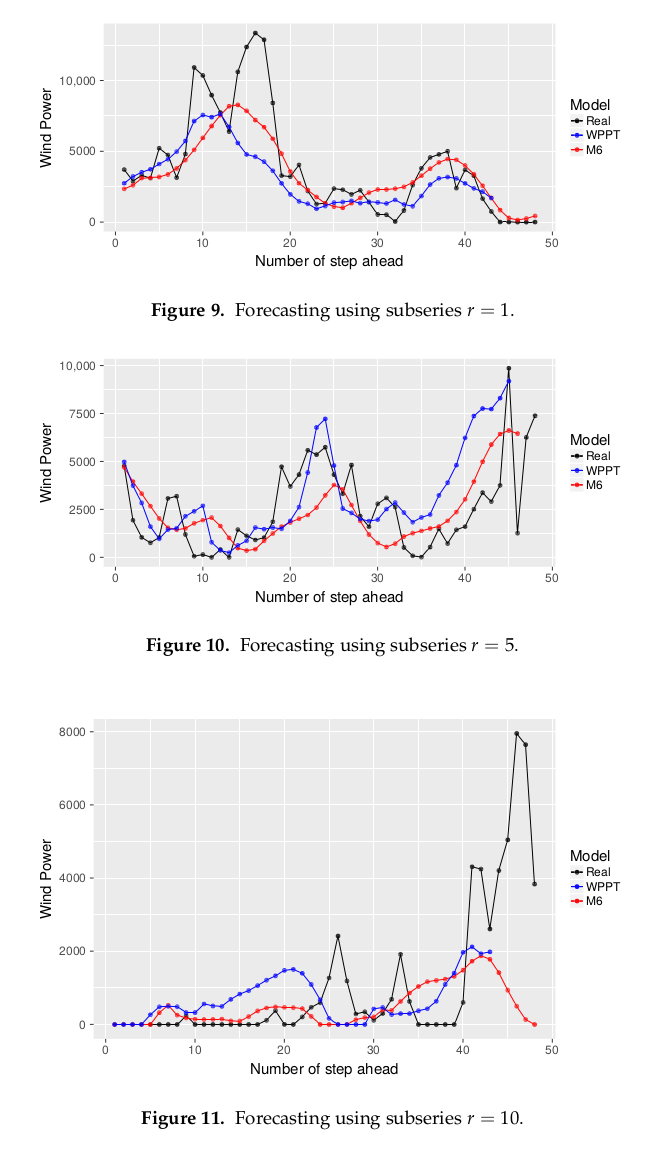
\includegraphics[width=\columnwidth]{lopez2018results}
  \caption{The results of 48-hour ahead predictions from a forecasting algorithm combining \gls{esn}
  and long short term memory algorithms (``M6''). Compared to the Wind Power Prediction
  Tool (WPPT). Figure reproduced from Lop\'ez et al. 2018
  \cite{lopez_wind_2018}.}
  \label{fig:lopez2018}
\end{figure}
